\chapter{Backgrounds}
\label{chap:backgrounds}

\section{Hardware Design Paradigms}
\label{sec:design-paradigm}

Traditional Register-Transfer Level (RTL) designs require hardware
designers to consider scheduling for all resources. During hardware
design, one has to ensure that any resource elements are correctly
employed, e.g., one should not write a register more than once in the
same cycle, which would cause incorrect assignment. If a particular
input port of a hardware component is used more than once, we do not
have any guarantees for the output value, also causing incorrect use
of values. A well-known RTL design framework, Verilog, lets users take
responsibility for this, thus one should carefully investigate if
there is an assignment which makes an incorrect state transition.
\begin{figure}[h]
  \centering
  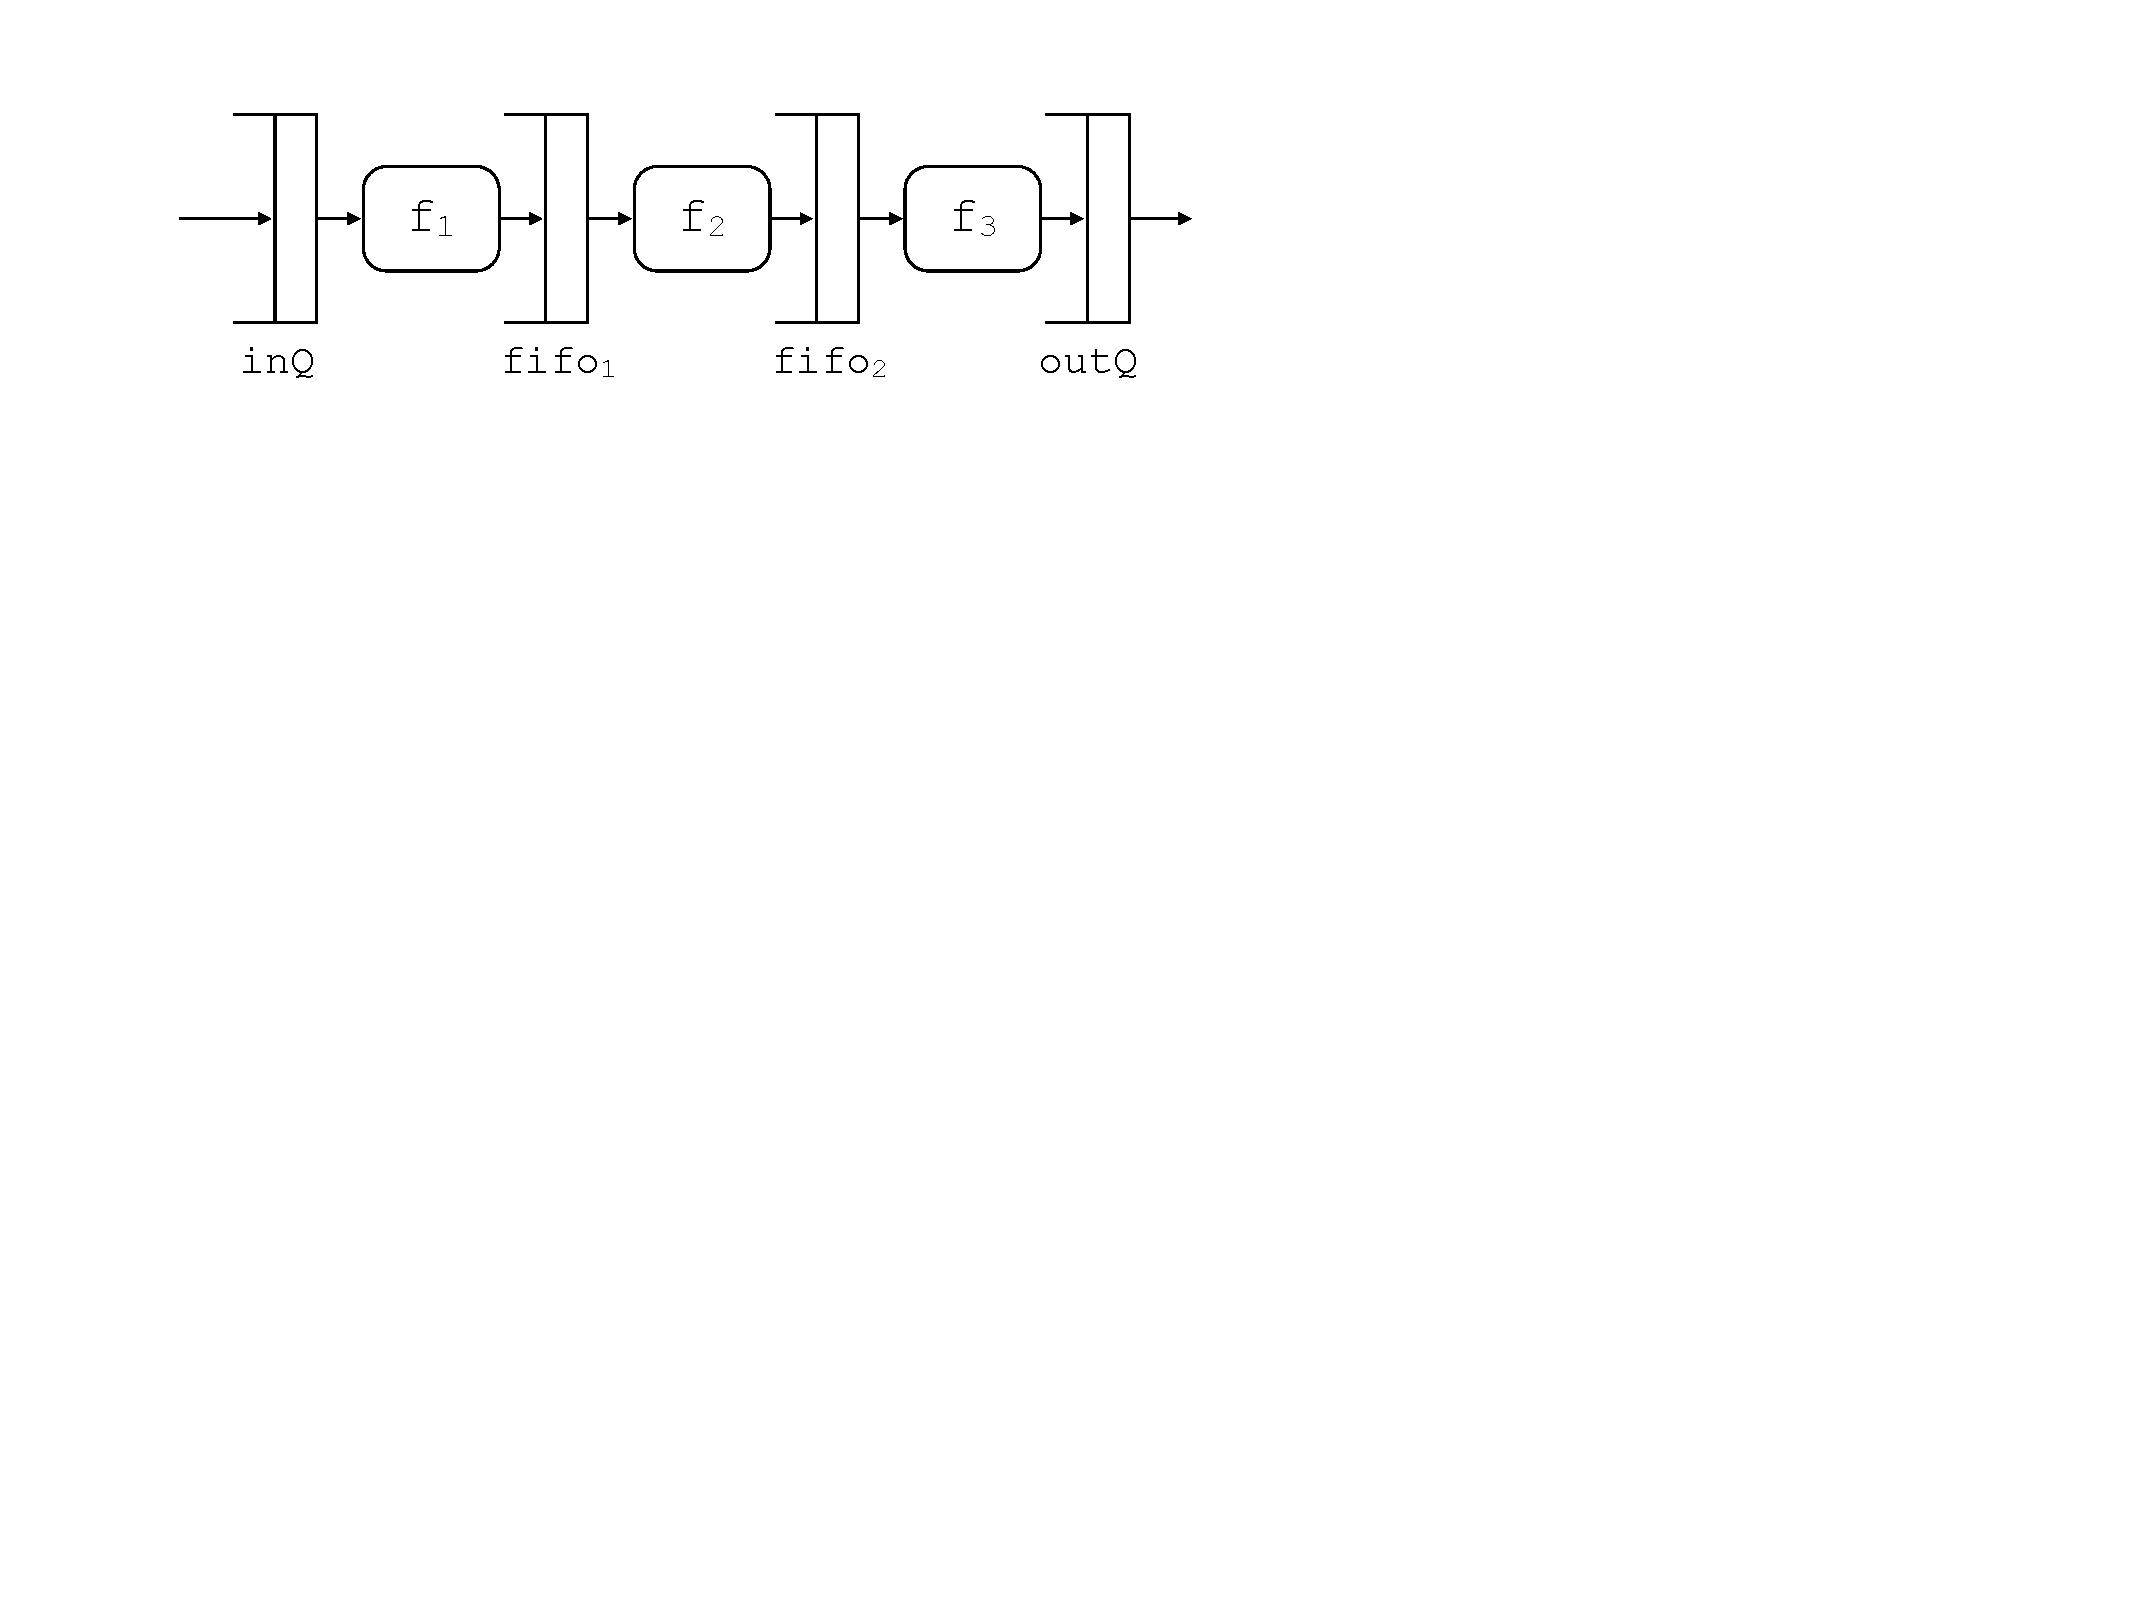
\includegraphics[width=0.5\textwidth]{figures/pipeline.pdf}
  \caption{A pipelined system}
  \label{fig-pipelined-system}
\end{figure}

A disadvantage of this approach is that having no separation between
functional parts and scheduling logic makes maintenance harder. Let us
revisit the pipelined system where three systems $f_1$, $f_2$, and
$f_3$ are connected by fifos, as shown in
\reffig{fig-pipelined-system}. For simplicity, suppose that only one
element can reside in a fifo. Since there is only one element in a
fifo, push and pop cannot be requested in the same cycle -- it will
cause double-write. Now the problem occurs because we have no
information whether push and pop will be requested simultaneously or
not. Thus in this case, we cannot avoid an implementation tightly
coupled with scheduling logic; for each case of push and pop, there is
no way for user except to define different implementations.

For this reason, in some frameworks like Verilog, designers tend to
specify the data path first, and then to define the controlling logic
which is entangled with the data path design. The problem with this
conventional design approach is that it is not flexible in perspective
of verification. If a designer specifies the controlling logic clearly
for a specific hardware system, it would be easy to verify
it. However, since that specification is only for one hardware system,
the verification approach used for the system may not be reusable for
other systems.

Guarded Atomic Action (GAA) is a design paradigm for correct and
effective scheduling that makes up for shortcomings of the RTL
designs. It is different from the traditional RTL designs mentioned
above. The main idea is that any hardware system has a (structural)
state component that can be captured by a set of variables that
represent registers or storage. State transition is done by a set of
rules, where a rule is a series of actions with \emph{guards} on this
state. A guard of a rule is a predicate that should be satisfied to
execute the rule. Each action (including one for rules) should be
atomic -- an execution of an action should be guaranteed to make a
state transition purely caused by the action.

\section{Semantics of the Bluespec Language}
\label{sec:bluespec-semantics}

\paragraph{Module structure}

Modularity forms the base semantics of the \Bluespec{} language. It is
simply to follow a natural hardware design concept. Hardware designers
usually design complex hardware components in a modular manner; small
module components are firstly designed, and they are composed to build
a large and complex one.

Bluespec also supports module definition. Each module has a set of
registers, called an \emph{internal state} of the module. The internal
state can be modified only by the module itself. In order to induce a
state change from the outside of the module, it should be requested by
method calls. The module also has a set of \emph{rules}. Each rule is
composed of GAAs. Rules are executed by a global rule scheduler. The
scheduler selects the maximal number of rules where the guards do not
conflict each others. Once the scheduler confirms the validity of the
guards, then they can be executed concurrently. Lastly, the module has
a set of \emph{methods}. Bluespec separates the notion of
\emph{Method} and \emph{ActionMethod}. Method is like a macro, which
evalutes an expression. From the perspective of hardware, Method can
be synthesized to a combinational circuit.  Whereas, ActionMethod is
composed of GAAs, and it only can be called by external modules. Thus,
it acts like an interface of the module, since ActionMethod is the
only way to manipulate internal states.

\begin{figure}[t]
  \centering{
    \begin{subfigure}[b]{0.5\textwidth}
      \bsvmodinst{PipelinedSystem}{inQ, fifo1, fifo2, outQ}{
        \bsvnone{\pgmrule}{stage0}{}{
          \pgmif{} \textrm{inQ.empty \&\& fifo1.notFull} \\
          \pgmthen{} \textrm{fifo1.enq(f0(inQ.first)); inQ.deq;}
        }\\
        \bsvnone{\pgmrule}{stage1}{}{
          \pgmif{} \textrm{fifo1.notEmpty \&\& fifo2.notFull} \\
          \pgmthen{} \textrm{fifo2.enq(f1(fifo1.first)); fifo1.deq;}
        }\\
        \bsvnone{\pgmrule}{stage2}{}{
          \pgmif{} \textrm{fifo2.notEmpty \&\& outQ.notFull} \\
          \pgmthen{} \textrm{outQ.enq(f2(fifo2.first)); fifo2.deq;}
        }\\
        \bsvnone{\pgmameth}{req}{(x)}{
          \textrm{inQ.enq(x);}
        }\\
        \bsvnone{\pgmameth}{res}{}{
          \pgmletin{x}{outQ.first}
          \textrm{outQ.deq;} \\
          \pgmret{x}
        }
      }
    \end{subfigure}
  }
  \caption{The pipelined system implemented with Bluespec}
  \label{ex-pipelined-system-bluespec}
\end{figure}

\reffig{ex-pipelined-system-bluespec} describes the psuedo-code
Bluespec module definition of the pipelined system shown in
\reffig{fig-pipelined-system}. The big module PipelinedSystem has four
module instances, named inQ, fifo1, fifo2, and outQ. It has three
rules (stage0, stage1, and stage2); each rule pulls an element from a
certain fifo, applies an operation, and push the resulting value into
the next fifo. The module has two interface methods: ``req'' is called
when there is a request with argument ``x'', and ``res'' is called to
get the result value.

\paragraph{Well-formedness of a module}

Syntactic correctness of a module does not imply the correct
execution. In other words, the module should satisfy an additional
number of conditions in order for valid execution. Firstly, a rule or
a method should not perform a write operation to the same register
twice (double-write). It also should not call the same method twice
(double-call). This is simply because actions in a rule (a method) are
executed simultaneously. A second condition is that method calls
cannot form a cycle among modules, since the cycle has no valid
behaviors in terms of hardware design. The last condition is that
register reads and writes should be defined within the module in which
the register is defined.

These conditions are sometimes called a well-formedness of a
module. It is usually defined independently with the semantics
definition, since it can be captured statically by traversing the
module definition. We formally define the well-formedness on
\refsect{sec-wf}, and use it on the correctness proof of an inlining
operation. See the section for more details.

\paragraph{Concurrent rule executions}

A guard of a rule includes which registers are written and which
methods are called. Since the guard contains conditions to execute the
rule, it is natural for the guard to have conditions for register
writes and method calls. If there are no explicit guard conditions on
the definition of the rule, then the guard only consists of register
and method conditions. The reason why guards contain such conditions
is to ensure there are no double-writes or double-calls during
multiple rule executions. Even if they are caught by forcing the
well-formedness condition, it is restricted within a rule or a
method. We cannot statically ensure if multiple rules can be executed
concurrently, without violating double-writes and double-calls.

Based on guards of rules, a rule scheduler tries to find a maximal set
of guards to be executed concurrently. The guards of concurrently
executed rules do not conflict each other. For instance, all the rules
of PipelinedSystem can be executed concurrently. In other words, the
rule scheduler can verify that the guards of the three rules in
PipelinedSystem do not conflict. This is because the rules do not
write the same register and do not call the same method.

\paragraph{One-rule-at-a-time semantics}

Multiple rule executions require an additional condition other than
non-conflicting guards, which is called the one-rule-at-a-time
semantics. The condition says that, multiple rules can be executed if
there \emph{exists a permutation of the rules} which yields the same
state change if they are executed sequentially. In other words, when
we define $(r_1; r_2; \cdots; r_n)$ be the concurrent execution of the
rules, then there exists $\{r_{p_1}, r_{p_2}, \cdots, r_{p_n}\}$, a
permutation of the rules, such that
\begin{center}
  \begin{math}
    (r_1; r_2; \cdots; r_n)(s) = r_{p_n}(\cdots(r_{p_2}(r_{p_1}(s)))\cdots).
  \end{math}
\end{center}

One-rule-at-a-time semantics makes verification easier. As the name
indicates, now it is fine to consider semantics where at most one rule
is executed at a time. Once we verify some properties under the
one-rule-at-a-time semantics, the whole system, in which a rule
scheduler is attached, also can be verified simply by proving that the
scheduler always selects rules based on the one-rule-at-a-time
semantics.

\section{Related Works: Previous Semantics Design}
\label{sec:related-works}

%% Nirav big-step semantics

%% Murali modular semantics

%% Any papers about inlining? Dan's thesis!! inlining used for merging
%% modules.

